%%%%%%%%%%%%%%%%%%%%%%%%%%%%%%%%%%%%%%%%%%%%%%%%%%%%%%%%%%%%%%%%%%%%%%%%%%%%%%%
%%                                                                           %%
%%   Dr Derek Harter                                                         %%
%%   Profesor, Department of Computer Science                                %% 
%%   Texas A&M University - Commerce, USA                                    %%
%%                                                                           %%
%%%%%%%%%%%%%%%%%%%%%%%%%%%%%%%%%%%%%%%%%%%%%%%%%%%%%%%%%%%%%%%%%%%%%%%%%%%%%%%
%%%%     SETTING STARTS - DO NOT CHANGE Unless your TeX setting require so   %%
%%%%%%%%%%%%%%%%%%%%%%%%%%%%%%%%%%%%%%%%%%%%%%%%%%%%%%%%%%%%%%%%%%%%%%%%%%%%%%%
%%----------------------------------------------------------------------------------
% DO NOT Change this. It is the required setting letterpaper page, 11pt, onside print, book style
%%----------------------------------------------------------------------------------
\documentclass[letterpaper,11pt,oneside]{book}

%%-------------------------------------
%% Page margin settings - % half inch margin all sides (recommended)
%%-------------------------------------
\usepackage[margin=1.2in]{geometry} 

%%-------------------------------------
%% Font settings - % CM San or Ariel (recommended)
%%-------------------------------------
% Switch the following two line off: to revert back to default LaTex font (NOT recommended)
\usepackage{amsfonts}
\renewcommand*\familydefault{\sfdefault}

%%-------------------------------------
%% Math/Definition/Theorem/Algorithm packages settings 
%%-------------------------------------
\usepackage[cmex10]{amsmath}
\usepackage{amssymb}
\usepackage{amsthm}
\newtheorem{mydef}{Definition}
\newtheorem{mytherm}{Theorem}

%%-------------------------------------
%% Algorithms/Code Listing environment settings  - 
%% Please do not change these settings
%%-------------------------------------
\usepackage{algorithm}
\usepackage{algpseudocode}
\renewcommand{\algorithmicrequire}{\textbf{Input:}}
\renewcommand{\algorithmicensure}{\textbf{Output:}}
\usepackage[utf8]{inputenc}
\usepackage{listings}
\usepackage{xcolor}
\definecolor{codegreen}{rgb}{0,0.6,0.1}
\definecolor{codegray}{rgb}{0.5,0.5,0.5}
\definecolor{codeblue}{rgb}{0.10,0.00,1.00}
\definecolor{codepurple}{rgb}{0.58,0,0.82}
\definecolor{backcolour}{rgb}{1.0,1.0,1.0}

\lstdefinestyle{mystyle}{
    backgroundcolor=\color{backcolour},   
    commentstyle=\color{codegreen},
    keywordstyle=\color{codeblue},
    numberstyle=\tiny\color{codegray},
    stringstyle=\color{codepurple},
    basicstyle=\ttfamily\footnotesize,
    breakatwhitespace=false,         
    breaklines=true,                 
    captionpos=b,                        
    keepspaces=true,                 
    numbers=left,                    
    numbersep=5pt,                  
    showspaces=false,                
    showstringspaces=false,
    showtabs=false,                  
    tabsize=2,
    frame=none
}
\lstset{style=mystyle}

%%-------------------------------------
%% Graphics/Figures environment settings
%%-------------------------------------
\usepackage{graphicx}
\usepackage{subfigure}
\usepackage{caption}
\usepackage{lipsum}

%%-------------------------------------
%% Table environment settings
%%-------------------------------------
\usepackage{multirow}
\usepackage{rotating}
\usepackage{makecell}
\usepackage{booktabs}
%\usepackage{longtable,booktabs}

%%-------------------------------------
%% List of Abbreviations settings
%%-------------------------------------
\usepackage{enumitem}
\newlist{abbrv}{itemize}{1}
\setlist[abbrv,1]{label=,labelwidth=1in,align=parleft,itemsep=0.1\baselineskip,leftmargin=!}

%%-------------------------------------
%% Bibliography/References settings   - Harvard Style was used in this report
%%-------------------------------------
\usepackage[hidelinks]{hyperref}
\usepackage[comma,authoryear]{natbib}
\renewcommand{\bibname}{References} % DO NOT remove or switch of 

%%-------------------------------------
%% Appendix settings     
%%-------------------------------------
\usepackage[toc]{appendix}
%%%%%%%%%%%%%%%%%%%%%%%%%%%%%%%%%%%%%%%%%%%%%%%%%%%%%%%%%%%%%%%%%%%%%%%%%%%%%%%%%%%%%%%
%%%%                     SETTING ENDS                                            %%%%%%
%%%%%%%%%%%%%%%%%%%%%%%%%%%%%%%%%%%%%%%%%%%%%%%%%%%%%%%%%%%%%%%%%%%%%%%%%%%%%%%%%%%%%%%
\begin{document}

    \captionsetup[figure]{margin=1.5cm,font=small,name={Figure},labelsep=colon}
    \captionsetup[table]{margin=1.5cm,font=small,name={Table},labelsep=colon}
    \SetLipsumDefault{1}
    
    \frontmatter
    
    \begin{titlepage}      
        \begin{center}
            
\includegraphics[width=3cm]{figures/tamuc-logo.png}\\[0.5cm]
            {\LARGE Texas A\&M University - Commerce\\[0.5cm]
            Department of Computer Science}\\[2cm]
			%{\color{blue} \rule{\textwidth}{1pt}}
			
			% -------------------------------
			% You need to edit some details here
			% -------------------------------  
            \linespread{1.2}\huge {
                %%%%%%%%%%%%%%%%%%%%%%%%%%%%
                %TODO: 1 TITLE of Your PROJECT 
                %%%%%%%%%%%%%%%%%%%%%%%%%%%%
                % chnage the following line  
                Stock Price Prediction Comparing by Transformers Neural Networks and ARIMA-ANN Hybrid
            }
            \linespread{1}~\\[2cm]
			%{\color{blue} \rule{\textwidth}{1pt}}
            {\Large 
                %%%%%%%%%%%%%%%%%%%%%%%%%%%%
                %TODO: 2 YOUR NAME
                %%%%%%%%%%%%%%%%%%%%%%%%%%%%             
                % chnage the following line
                Sridhar Chithathuru
                % change end             
            }\\[1cm] 
            

            {\large 
                %%%%%%%%%%%%%%%%%%%%%%%%%%%%
                %TODO: 3 YOUR NAME Supervisor's name(s)
                %%%%%%%%%%%%%%%%%%%%%%%%%%%%             
                % change the following line                
                \emph{Supervisor:} Derek Harter, Ph.D.}\\[1cm] % if applicable
            
    		% PLEASE DO NOT CHANGE THIS TEXT %
            \large A report submitted in partial fulfilment of the requirements of\\Texas A\&M University - Commerce for the degree of\\ Master of Science in \textit{Computer Science}\\[0.3cm] 
            \vfill
            
            
            \today % Please update this date you can use \date{April 2020} for fixed date
        \end{center}
    \end{titlepage}
    
    
    % -------------------------------------------------------------------
    % Declaration
    % -------------------------------------------------------------------
    \newpage
    \thispagestyle{empty}
    \chapter*{\Large Declaration}
    % PLEASE CHANGE THIS TEXT EXCEPT YOUR NAME%
    % -------------------------------
    %TODO: PLEASE ONLY UPDATE HERE -- PLEASE WRITE YOUR NAME %    
    % ------------------------------- 
    I,
    %%%%%%%%%%%%%%%%%%%%%%%
     Sridhar Chithathuru, % Mandatory part
    %%%%%%%%%%%%%%%%%%%%%%%
    of the Department of Computer Science, Texas A\&M University - Commerce, confirm that this is my own work and figures, tables, equations, code snippets, artworks, and illustrations in this report are original and have not been taken from any other person's work, except where the works of others have been explicitly acknowledged, quoted, and referenced. I understand that if failing to do so will be considered a case of plagiarism. Plagiarism is a form of academic misconduct and will be penalised accordingly. \\
    
    %% Please delete as appropriate. 
    \noindent
    %%%%%%%%%%%%%%%%%%%%%%%%%%%%%%%%%%%%%%%%%%%%%%% 
    %TODO 1 Consent for example copy -  we will use 
    I give consent to a copy of my report being shared with future students as an exemplar. \\
    
    \noindent
    %%%%%%%%%%%%%%%%%%%%%%%%%%%%%%%%%%%%%%%%%%%%%%% 
    %TODO 2 Consent to let the report to use use by library for public use
    I give consent for my work to be made available more widely to members of TAMUC and public with interest in teaching, learning and research. 
    %%%%%%%%%%%%%%%%%%%%%%%%%%%%%%%%%%%%%%%%%%%%%%%
    ~\\[1cm]
    \begin{flushright}
	%------------------------------ 
	% change the following line
    %TODO: PLEASE UPDATE  Your Name  -------------------------------%
	Sridhar Chithathuru % Please change it to your name
    
    \today
    \end{flushright}

     
    % -------------------------------------------------------------------
    % Abstract and Acknowledgement
    % -------------------------------------------------------------------
    
    %Two resources useful for abstract writing.
% Guidance of how to write an abstract/summary provided by Nature: https://cbs.umn.edu/sites/cbs.umn.edu/files/public/downloads/Annotated_Nature_abstract.pdf %https://writingcenter.gmu.edu/guides/writing-an-abstract
\chapter*{\center \Large  Abstract}
%%%%%%%%%%%%%%%%%%%%%%%%%%%%%%%%%%%%%%
% Replace all text with your text
%%%%%%%%%%%%%%%%%%%%%%%%%%%%%%%%%%%

The economic condition of traders, customers, and financial institutions has been significantly 
influenced by the finance sector. With the use of cutting-edge deep learning and machine 
learning algorithms, artificial intelligence such as deep learning are having significant impacts in finance. Deep 
learning and machine learning models are used by traders and investors to predict the movements 
of financial instruments. Investment methods in the stock market are intricate and depend on a 
thorough analysis of a large quantity of data. The Yahoo-finance dataset \citep{dataset} displays many firm 
aspects for stocks, news, quotations, and other items for every potential shift across time. 
Using transformers and ARIMA-ANN, we build a model that predicts prices at each instant of time. 


    % -------------------------------------------------------------------
	% Acknowledgement
	% -------------------------------------------------------------------
   
    \chapter*{\center \Large  Acknowledgements}
%%%% Update with your text %%%%%%%%%%%%%%%
An acknowledgements section is optional. You may like to acknowledge the support and help of your supervisor(s), friends, or any other person(s), department(s), institute(s), etc. If you have been provided specific facility from department/school acknowledged so.  

   
    
    % -------------------------------------------------------------------
    % Contents, list of figures, list of tables
    % -------------------------------------------------------------------
    
    \tableofcontents
    \listoffigures
    \listoftables
    \chapter*{List of Abbreviations}
\chaptermark{List of Abbreviations}
%%%%%%%%%%%%%%%%%%%%%%%%%%%%%%%%%%%
%%  Enter your list of Abbreviation and Symbols in this file
%%%%%%%%%%%%%%%%%%%%%%%%%%%%%%%%%%%
\begin{abbrv}
    
    \item[SMPCS]			School of Mathematical, Physical and Computational Sciences
    
\end{abbrv}
 %  Enter your list of Abbreviation and Symbols in this file
    
    %%%%%%%%%%%%%%%%%%%%%%%%%%%%%%%%%%%%%%%%%%%%%%%%%%%%%%%%%%%%%%%%%%%%%%%%
    %%                                                                    %%  
    %%  Main chapters and sections of your project                        %%  
    %%  Everything from here on needs updates in your own words and works %%
    %%                                                                    %%
    %%%%%%%%%%%%%%%%%%%%%%%%%%%%%%%%%%%%%%%%%%%%%%%%%%%%%%%%%%%%%%%%%%%%%%%%
    \mainmatter
    % Read for preparation of document in LaTex 
    % Lamport, L. (1986), LATEX: A Document Preparation System, Addison-Wesley.
    
    \chapter{Introduction}
\label{ch:into} % This how you label a chapter and the key (e.g., ch:into) will be used to refer this chapter ``Introduction'' later in the report. 
% the key ``ch:into'' can be used with command \ref{ch:intor} to refere this Chapter.

\textbf Stockbrokers, traders, and investors that purchase, sell, or share transactions collectively make up the stock market. Because so many businesses post their stock lists online, investors find their stocks appealing \cite{bhattacharjee2019stock}. The size of the markets and the speed at which deals are completed now make it impractical for investors to use their own experience, which they once used to discern market trends. A nation's economic status affects a number of industries, including investment banking, metals, agriculture, and finance, either directly or indirectly. The fundamental law of supply and demand dictates that the growth of these industries depends on their volatility. Due to the fact that investors have been attempting various methods since the 16s in order to increase the returns on their investments by learning about various firms \cite{mehta2021stock}. There is a noticeable increase in demand for stock market. Because of the exceptional revenues, as we all know, it has been in the news for a long time. Accurately predicting future financial outcomes is the main goal of stock price prediction. Machine Learning algorithms have shown promise in a number of sectors in recent years, and as a result, many traders are using these strategies in their particular domains. 


An accounting forecast can be viewed as a difficult time-varying prediction. A transformer in deep learning is a model that uses the self-attention process and weights each incoming data component differently based on its significance. Transformers are intended to evaluate sequential input data, including plain language, much like recurrent neural networks (RNNs). But transformers handle the whole input all at once, unlike RNNs. The statistical prediction instruments that have been most widely used are ARIMA models. Though regrettably, not all future occurrences are predicted by this model with the same level of accuracy. This is because, following three or four predicted values, the forecasts converge to the series mean. Usually, the maximum likelihood model or the least squares estimation model are used to estimate the parameters of ARIMA models. In several disciplines, most notably economics, artificial neural networks (ANNs) have been utilized for prediction. 

After being first presented by a group of researchers at Google Brain in 2017, transformers are quickly displacing RNN models, such as extended short-term memory, as the preferred model for problems with natural language processing (LSTM). White and Safi (2016) demonstrated that when the ANN model's linking function was nonlinear, it outperformed the ARIMA model. But the ARIMA model did better than the ANN model when its linking function was linear. This is not unexpected given that the ARIMA model was created especially for this circumstance \cite{safi2021hybrid}. The hybrid model that is employed is a blend of the autoregressive integrated moving average (ARIMA) model, the nonlinear artificial neural network (ANN), and the Error, Trend, and Seasonality (ETS) models. It is a linear stochastic model. The hybrid model outperforms the linear and nonlinear models, according to data from earlier investigations. For instance, the hybrid model was shown to have the highest accuracy when used to forecast drought in India using a standardized precipitation index series, in comparison to separate stochastic and ANN models.

We use the Y-finance dataset to forecast a single ticker, taking into account several factors such as volume, high, close, and open. Utilizing nine tickers, we are able to achieve prediction characteristics whereby the tenth ticker is anticipated by utilizing all nine ticker values. To achieve these kinds of significant modifications, we approximate a method wherein the model's prediction weights produce the particular shift in testing and prediction values. Ultimately, based on the kind of algorithm selected and developed, a general comparison analysis using various time instances is confirmed. 

%%%%%%%%%%%%%%%%%%%%%%%%%%%%%%%%%%%%%%%%%%%%%%%%%%%%%%%%%%%%%%%%%%%%%%%%%%%%%%%%%%%
\section{Background}
\label{sec:into_back}
Describe to a reader the context of your project. That is, what is your project and what its motivation. Briefly explain the major theories, applications, and/or products/systems/algorithms whichever is relevant to your project.

\textbf{Cautions:} Do not say you choose this project because of your interest, or your supervisor proposed/suggested this project, or you were assigned this project as your final year project. This all may be true, but it is not meant to be written here.

%%%%%%%%%%%%%%%%%%%%%%%%%%%%%%%%%%%%%%%%%%%%%%%%%%%%%%%%%%%%%%%%%%%%%%%%%%%%%%%%%%%
\section{Problem statement}
\label{sec:intro_prob_art}
Given the available computing power and training constraints, is it possible to build and train both Transformer Neural Networks and the ARIMA-ANN hybrid model using historical stock price data? What distinguishes Transformer Neural Networks' stock price prediction skills from those of the ARIMA-ANN hybrid model, and what are their distinctive characteristics and performance metrics? What insights can be acquired on the capacity of these models to adjust to shifting market conditions, and how does the selection of prediction model affect the process of making investments over a certain time period?

%%%%%%%%%%%%%%%%%%%%%%%%%%%%%%%%%%%%%%%%%%%%%%%%%%%%%%%%%%%%%%%%%%%%%%%%%%%%%%%%%%%
\section{Aims and objectives}
\label{sec:intro_aims_obj}
Describe the ``aims and objectives'' of your project. 

\textbf{Aims:} The aims tell a read what you want/hope to achieve at the end of the project. The  aims define your intent/purpose in general terms.  

\textbf{Objectives:} The objectives are a set of tasks you would perform in order to achieve the defined aims. The objective statements have to be specific and measurable through the results and outcome of the project.



%%%%%%%%%%%%%%%%%%%%%%%%%%%%%%%%%%%%%%%%%%%%%%%%%%%%%%%%%%%%%%%%%%%%%%%%%%%%%%%%%%%
\section{Solution approach}
\label{sec:intro_sol} % label of Org section
Briefly describe the solution approach and the methodology applied in solving the set aims and objectives.

Depending on the project, you may like to alter the ``heading'' of this section. Check with you supervisor. Also, check what subsection or any other section that can be added in or removed from this template.

\subsection{A subsection 1}
\label{sec:intro_some_sub1}
You may or may not need subsections here. Depending on your project's needs, add two or more subsection(s). A section takes at least two subsections. 

\subsection{A subsection 2}
\label{sec:intro_some_sub2}
Depending on your project's needs, add more section(s) and subsection(s).

\subsubsection{A subsection 1 of a subsection}
\label{sec:intro_some_subsub1}
The command \textbackslash subsubsection\{\} creates a paragraph heading in \LaTeX.

\subsubsection{A subsection 2 of a subsection}
\label{sec:intro_some_subsub2}
Write your text here...

%%%%%%%%%%%%%%%%%%%%%%%%%%%%%%%%%%%%%%%%%%%%%%%%%%%%%%%%%%%%%%%%%%%%%%%%%%%%%%%%%%%
\section{Summary of contributions and achievements} %  use this section 
\label{sec:intro_sum_results} % label of summary of results
Describe clearly what you have done/created/achieved and what the major results and their implications are. 


%%%%%%%%%%%%%%%%%%%%%%%%%%%%%%%%%%%%%%%%%%%%%%%%%%%%%%%%%%%%%%%%%%%%%%%%%%%%%%%%%%%
\section{Organization of the report} %  use this section
\label{sec:intro_org} % label of Org section
Describe the outline of the rest of the report here. Let the reader know what to expect ahead in the report. Describe how you have organized your report. 

\textbf{Example: how to refer a chapter, section, subsection}. This report is organised into seven chapters. Chapter~\ref{ch:lit_rev} details the literature review of this project. In Section~\ref{ch:method}...  % and so on.

\textbf{Note:}  Take care of the word like ``Chapter,'' ``Section,'' ``Figure'' etc. before the \LaTeX command \textbackslash ref\{\}. Otherwise, a  sentence will be confusing. For example, In \ref{ch:lit_rev} literature review is described. In this sentence, the word ``Chapter'' is missing. Therefore, a reader would not know whether 2 is for a Chapter or a Section or a Figure.


    \chapter{Literature Review}
\label{ch:lit_rev} %Label of the chapter lit rev. The key ``ch:lit_rev'' can be used with command \ref{ch:lit_rev} to refer this Chapter.

Bitcoin, a decentralized digital currency, has become more well-known as a substitute for stock market investing. Numerous dangers and factors have the potential to impact the stock market. However, bitcoin is one cryptocurrency that has been steadily increasing in value over the past several years, despite the fact that the value of other cryptocurrencies might suddenly crash without anybody being able to explain why. The stock market requires forecasts about bitcoin from both a human analyst and an automated software because to its volatility. 

Traders are eager to capitalize on the opportunities presented by the thriving Indian stock market at the moment. Because of this, it is important to estimate the Nifty 50's value accurately while trading stocks. The futures and options (F\&O) market component is one of the fundamental indicators of the Nifty 50.Machine learning techniques are used for more precise prediction. The forward neural network, the generalized regression neural network, the radial basis neural network, and the precise radial basis neural network are the four machine-learning-based neural network models we discuss in this study. By comparing the Nifty 50 value with a minimum error rate, four models were offered in the study effort to anticipate the degree of accuracy. In order to finish the research, samples were gathered from the Yahoo Finance website spanning the previous nine years, from January 2013 to June 2021. The original beginning value, day high, day low, and total volumes traded on that day are all considered input characteristics for the Nifty 50 value of the stock market. An output parameter is utilized, which is the day's closing value. The testing results demonstrate that the radial basis neural network model outperforms the other three models with an accuracy of 98.17\%, making it the best model for predicting the Nifty 50 stock market perspectives \cite{lamba2021comparative}.


% PLEAE CHANGE THE TITLE of this section
\section{Example of in-text citation of references in \LaTeX} 
% Note the use of \cite{} and \citep{}
The references in a report relate your content with the relevant sources, papers, and the works of others. To include references in a report, we \textit{cite} them in the texts. In MS-Word, EndNote, or MS-Word references, or plain text as a list can be used. Similarly, in \LaTeX, you can use the ``thebibliography'' environment, which is similar to the plain text as a list arrangement like the MS word. However, In \LaTeX, the most convenient way is to use the BibTex, which takes the references in a particular format [see references.bib file of this template] and lists them in style [APA, Harvard, etc.] as we want with the help of proper packages.    

These are the examples of how to \textit{cite} external sources, seminal works, and research papers. In \LaTeX, if you use ``\textbf{BibTex}'' you do not have to worry much since the proper use of a bibliographystyle package like ``agsm for the Harvard style'' and little rectification of the content in a BiBText source file [In this template, BibTex are stored in the ``references.bib'' file], we can conveniently generate  a reference style. 

Take a note of the commands \textbackslash cite\{\} and \textbackslash citep\{\}. The command \textbackslash cite\{\} will write like ``Author et al. (2019)'' style for Harvard, APA and Chicago style. The command \textbackslash citep\{\} will write like ``(Author et al., 2019).'' Depending on how you construct a sentence, you need to use them smartly. Check the examples of \textbf{in-text citation} of sources listed here [This template recommends the \textbf{Harvard style} of referencing.]:
\begin{itemize}
    \item \cite{lamport1994latex} has written a comprehensive guide on writing in \LaTeX ~[Example of \textbackslash cite\{\} ].
    \item If \LaTeX~is used efficiently and effectively, it helps in writing a very high-quality project report~\citep{lamport1994latex} ~[Example of \textbackslash citep\{\} ].   
    \item A detailed APA, Harvard, and Chicago referencing style guide are available in~\citep{uor_refernce_style}.
\end{itemize}

\noindent 
Example of a numbered list:
\begin{enumerate}
    \item \cite{lamport1994latex} has written a comprehensive guide on writing in \LaTeX.
    \item If \LaTeX is used efficiently and effectively, it helps in writing a very high-quality project report~\citep{lamport1994latex}.   
\end{enumerate}

% PLEAE CHANGE THE TITLE of this section
\section{Example of ``risk'' of unintentional plagiarism}
Using other sources, ideas, and material always bring with it a risk of unintentional plagiarism. 

\noindent
\textbf{\color{red}MUST}: do read the university guidelines on the definition of plagiarism as well as the guidelines on how to avoid plagiarism~\citep{uor_plagiarism}.




% A possible section of you chapter
\section{Critique of the review} % Use this section title or choose a betterone
Describe your main findings and evaluation of the literature. ~\\

% Pleae use this section
\section{Summary} 
Write a summary of this chapter~\\
% https://guides.library.bloomu.edu/litreview
    \chapter{Algorithms}

Neural networks are a set of algorithms that identify patterns and are roughly modeled after the human brain. They use machine perception to categorize or organize raw information in order to better interpret sensory data. All real-world data, including pictures, sounds, texts, and time series, must be transformed into vectors in order to understand the numerical patterns inherent therein.

\section{Design Procedure} %  use this section 
\label{sec:intro_sum_results} % label of summary of results
                  
        Step 1: First, generate the dataset using the custom function from the y-finance package. &    \\        
        Step 2: Begin the solution feature extraction for 9 tickers with 1 ticker as the feature model.  &    \\        
        Step 3:Indicate the total selected and merged samples based on the multi-objective function with regard to the single ticker chosen.   &    \\
        Step 4: Normalize the entire data to improve accuracy and intuitive learning responses.  &    \\
        Step 5:Determine the overall featured labels, then design a TNN and ARIMA-ANN model for training.      &    \\
        Chapter 6 & Conclusions and Future Work  &    \\        
        Step 7: Visualize the data using 5 minute, 1 hour, and 1 day increments. &    \\      
        Step 8:Show the total error change on the single ticker using the appropriate highlighted data as (open (1 ticker)-open (9 tickers)).  & \\
Step 9:How the proposed and current algorithms affect the display of stock data dependent on the year. & \\

\section{Transformer Neural Networks}
In many neural network topologies, the transformer is used to handle sequential data such as natural language text, genetic sequences, auditory signals, or time series data. Transformer neural networks are most commonly employed for natural language processing. A transformer neural network can convert an input phrase as a series of vectors into an encoding vector, which it can then decode back into a sequence of vectors. The attention mechanism is an important component of the transformer. The attention mechanism determines the significance of other tokens in an input for encoding a certain token. The attention mechanism in a machine translation model, for example, allows the transformer to convert words such as "it" into a word of the proper gender in French or Spanish by paying attention to all relevant phrases in the original text. Importantly, the transformer may use the attention mechanism to determine how to translate a word by concentrating on phrases to the left and right of the current sentence. Transformer neural networks have replaced the previously used recurrent neural network (RNN), long short-term memory (LSTM), and gated recurrent (GRU) neural network designs.

Importantly, the transformer may use the attention mechanism to select how to translate a word by focusing on certain phrases to the left and right of the current sentence. Transformer neural networks have taken the role of previous neural network architectures such as recurrent neural network (RNN), long short-term memory (LSTM), and gated recurrent (GRU).

\section {Transformer Neural Network Design}

\begin{figure}[ht]
    \centering
    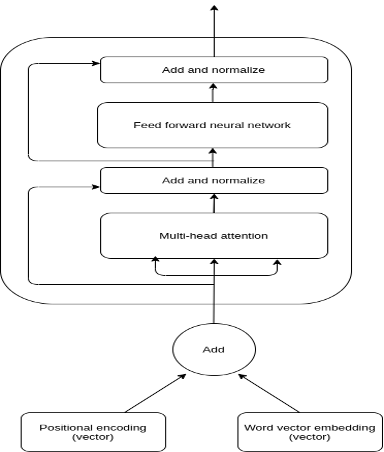
\includegraphics[scale=0.7]{figures/Transformer.png}
    \caption{The architecture of a transformer neural network.}
    \label{fig:chart_a}
\end{figure}

The transformer neural network takes a phrase as input and divides it into two sequences: one with word vector embeddings and one with positional encodings. The text is represented mathematically using word vector embeddings. Words must first be translated to embedding format before they can be processed by a neural network. In the embedding representation, each dictionary word is represented by a vector. Positional encodings are vector representations of the word's original location inside the sentence.The transformer combines word vector embeddings and positional encodings before passing the resulting data through a variety of encoders and decoders. It should be emphasized that, unlike RNNs and LSTMs, the entire input is sent into the network at once, rather than one piece at time.

Each encoder converts the input into a new collection of vectors known as an encoding. The decoders do the inverse, turning the encodings into a set of probabilities for possible output words. The SoftMax function may be used to represent the output probabilities in another natural language phrase. The attention mechanism, which is included in all encoders and decoders, allows the processing of one input word to integrate relevant data from other words while masking the words that do not contain significant information. This must be calculated several times, thus we use the parallel computing capabilities given by GPUs to build various attention strategies. The multi-head attention mechanism is to blame. Transformers have an advantage over LSTMs and RNNs in that they can analyze many words at the same time.




\section{Autoregressive Integrated Moving Average (ARIMA)}

It is a statistical analysis model that uses time series data to either better comprehend the data or forecast future trends. A statistical model is autoregressive if it predicts future values based on previous values. For example, an ARIMA model may attempt to estimate a stock's future pricing based on its past performance or a company's earnings based on previous periods.

ARIMA's components serve as parameters using standard notation. A conventional nomenclature for ARIMA models is ARIMA with p, d, and q, where integer values represent the parameters to denote the kind of ARIMA model utilized. Parameters can be specified as: 1
\begin{figure}[ht]
    \centering
    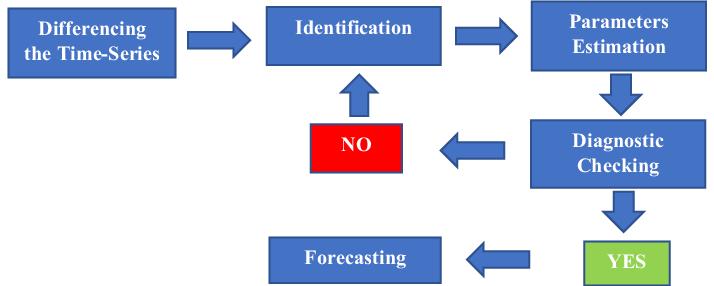
\includegraphics[scale=0.5]{figures/Arima.png}
    \caption{The architecture of a ARIMA neural network.}
    \label{fig:chart_a}
\end{figure}

p is the number of lag observations in the model, commonly known as the lag order.
d: the number of times the raw observations are differentiated; also known as the degree of differencing.
q is the size of the moving average window, commonly known as the moving average's order.
To start creating an ARIMA model for an investment, you download as much price data as possible. After identifying the data patterns, you look at the autocorrelations to determine the lowest order of differencing (d). If the lag-1 autocorrelation is zero or negative, the series is already differentiated. If the lag-1 is more than zero, you may need to differentiate the series further.

Next, compare autocorrelations and partial autocorrelations to establish the order of regression (p) and the order of the moving average. Once you have the necessary information, you may pick the model you will use.

\section{Artificial Neural Networks (ANN)}
Artificial Neural Networks (ANN) are algorithms that simulate brain activity and are used to model complex patterns and foresee problems. The Artificial Neural Network (ANN) is a deep learning technique based on the notion of biological neural networks in the human brain. An attempt to imitate the workings of the human brain led to the development of artificial neural networks (ANN). ANNs operate very similarly to biological neural networks, however they are not identical. The ANN algorithm only takes numbers and structured input.

\begin{figure}[ht]
    \centering
    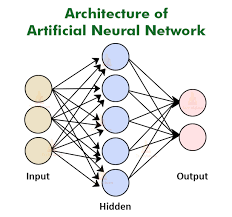
\includegraphics[scale=1]{figures/ANN.png}
    \caption{The architecture of a ANN neural network.}
    \label{fig:chart_a}
\end{figure}

Image, Text, and Speech are examples of unstructured and non-numeric data types that are accepted by Convolutional Neural Networks (CNN) and Recursive Neural Networks (RNN). This page only discusses Artificial Neural Networks. The majority of neural networks have units that connect one layer to the next. Each of these links has a weight, which determines how one unit affects another. As input is sent from one unit to another, the neural network learns more about the data, finally producing an output from the output layer. 










    \chapter{Results}
\label{ch:results}
The Anaconda Platform is used for overall design and implementation on the MAC Book Pro. We created six Python files that show the overall changes from 5 minutes, 1 hour, and 1 day for the ARIMA-ANN Hybrid and TNN algorithms. The design includes argument analysis for code execution for each type of firm, and the calling feature is more user-friendly. The ARIMA-ANN hybrid design was carried out with ARIMA parameters (2,1,3), and for TNN, we used 2-layer Dense modeling for encoder and decoder, as shown in Algorithm 1. The total experiment on timeseries prediction was carried out based on the numerous functional elements indicating the time features of the Yahoo finance stocks for the advancement.The goal of this paper is to provide a solution that will predict Yahoo's total stock price, suggesting the best prediction method.

The design models are executed in two stages for each form of effective inquiry, one representing the prediction time values for the stocks and the other reflecting the overall effective loss observed variation on each type of company, assuring the corrected next day projected value.

\section{Comparision of Algorithms}
Based on the predicted values accuracy,  calculated mean square error and considering the time taken to calculate the stock values of the given input company Transformer neural network performs better in the current scenario in both predicting the values and time taken for calculations with less RMSE value compared to ARIMA-ANN hybrid. ARIMA-ANN hybrid also performs well to calculate the stock values but while training ANN part of the model, it consumes more time for calculations. 
In light of this, we may conclude that the Transformer neural network outperformed all others in terms of stock price prediction for a particular ticker.

The following images are the results from the model regarding predicting the values of next day stock.

\begin{figure}[ht]
    \centering
    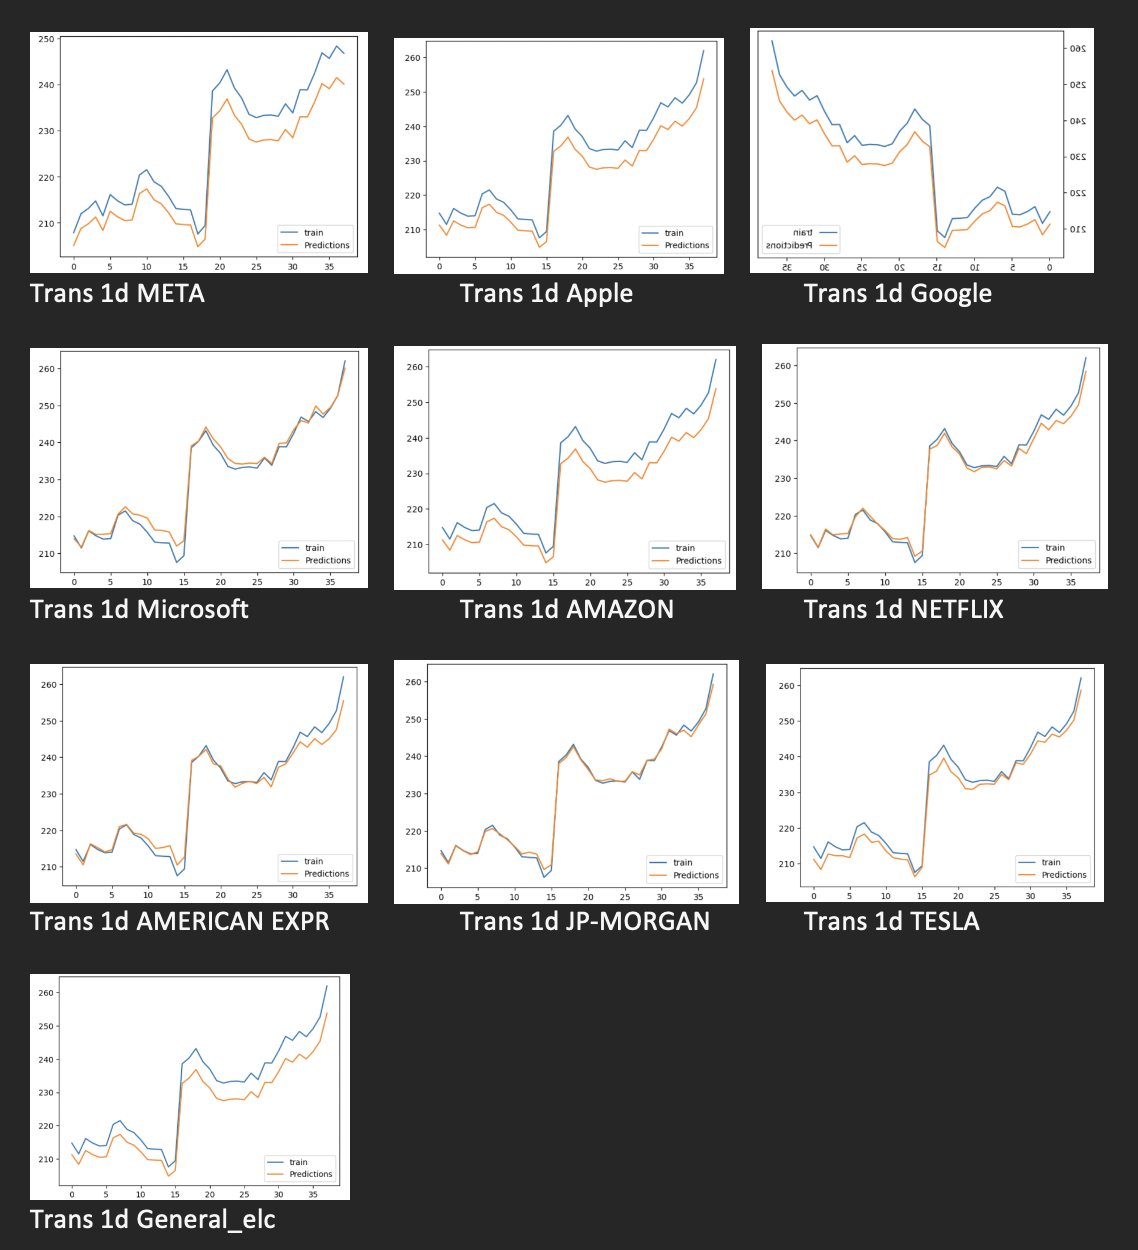
\includegraphics[scale=0.2]{figures/Trans 1d.png}
    \caption{Representing the overall actual and predicted values for Close stock for TNN algorithms with time period as 1d.}
    \label{fig:chart_b}
\end{figure}
\textbf 

\begin{figure}[ht]
    \centering
    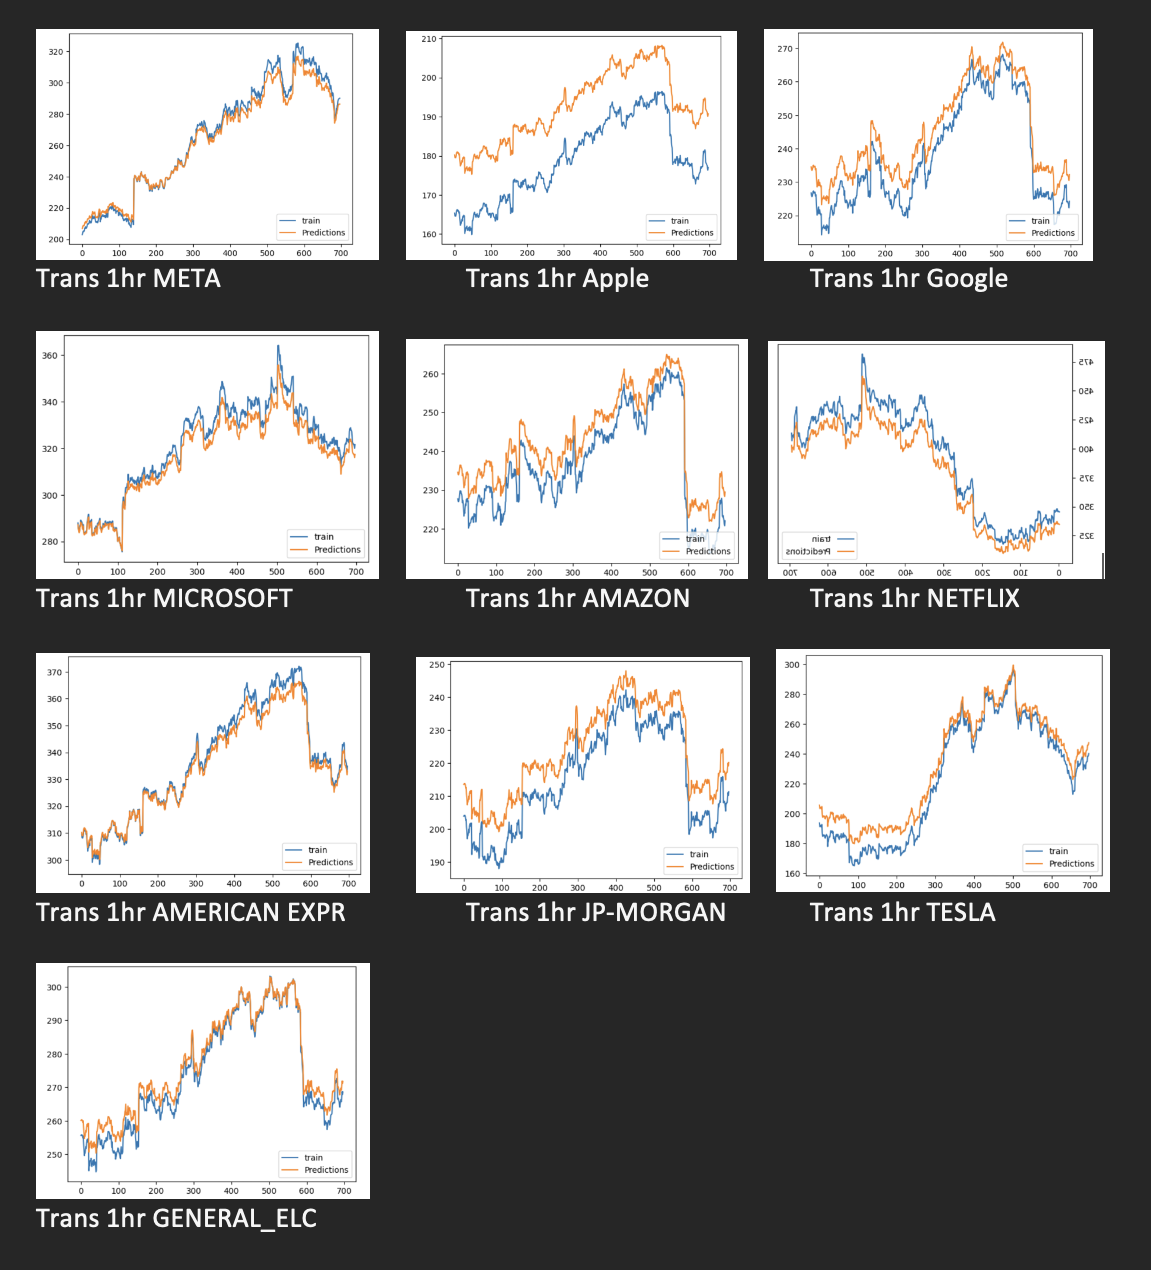
\includegraphics[scale=0.2]{figures/Trans 1hr.png}
    \caption{Representing the overall actual and predicted values for Close stock for TNN algorithms with time period as 1hr.}
    \label{fig:chart_a}
\end{figure}

\begin{figure}[ht]
    \centering
    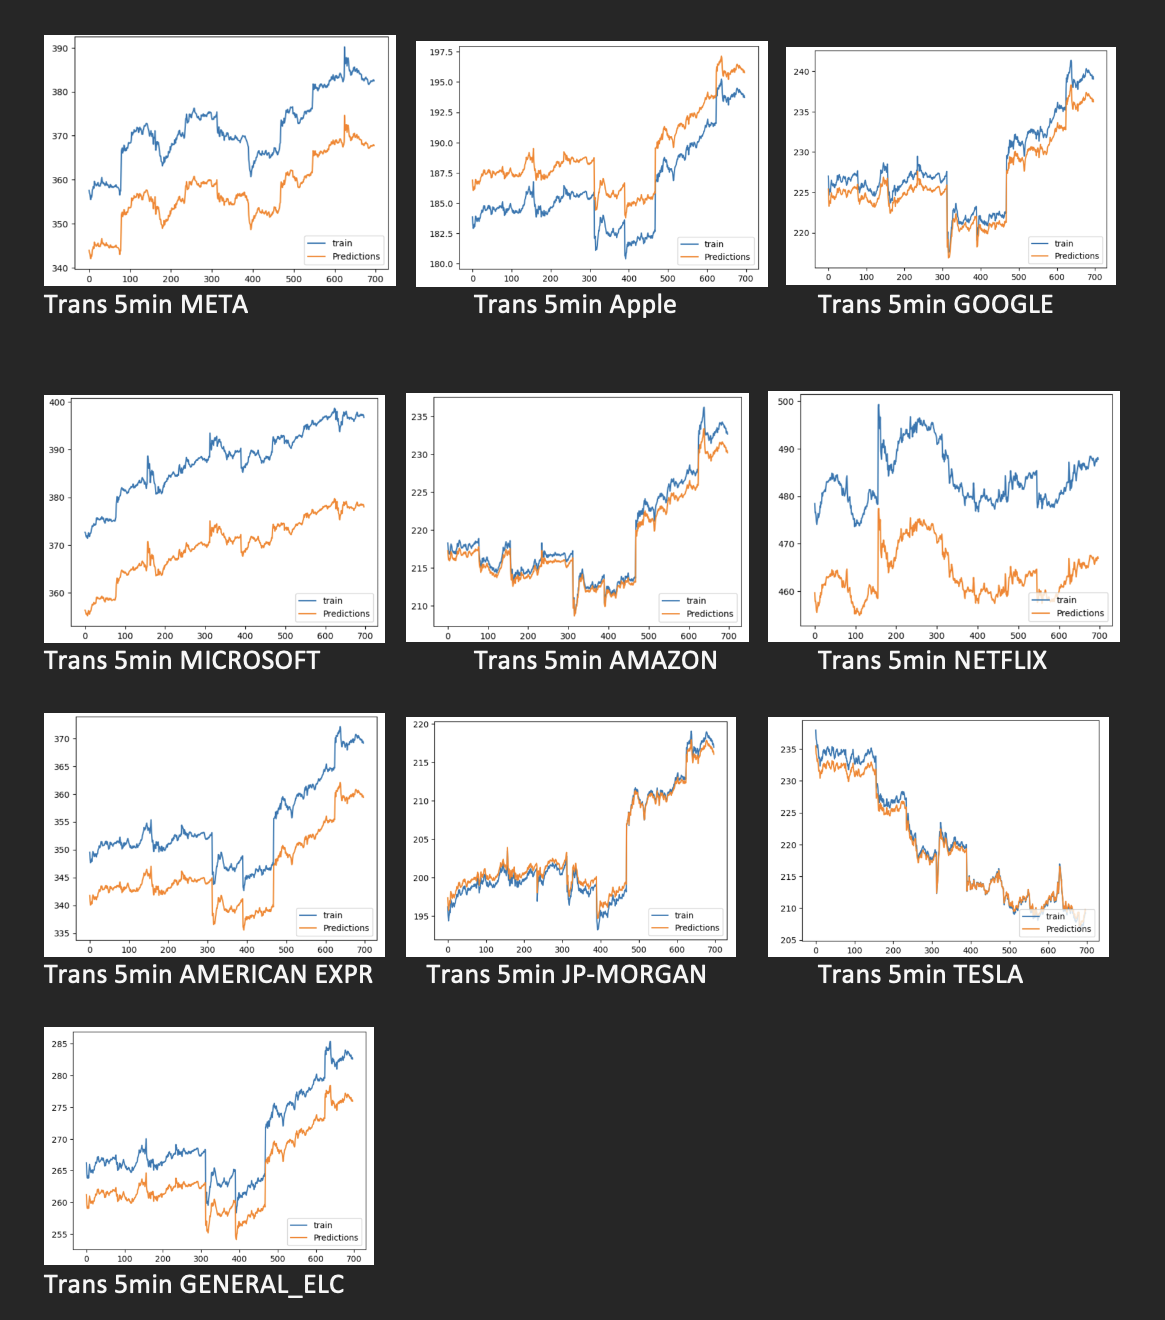
\includegraphics[scale=0.2]{figures/Trans 5min.png}
    \caption{Representing the overall actual and predicted values for Close stock for TNN algorithms with time period as 5min.}
    \label{fig:chart_c}
\end{figure}

\begin{figure}[ht]
    \centering
    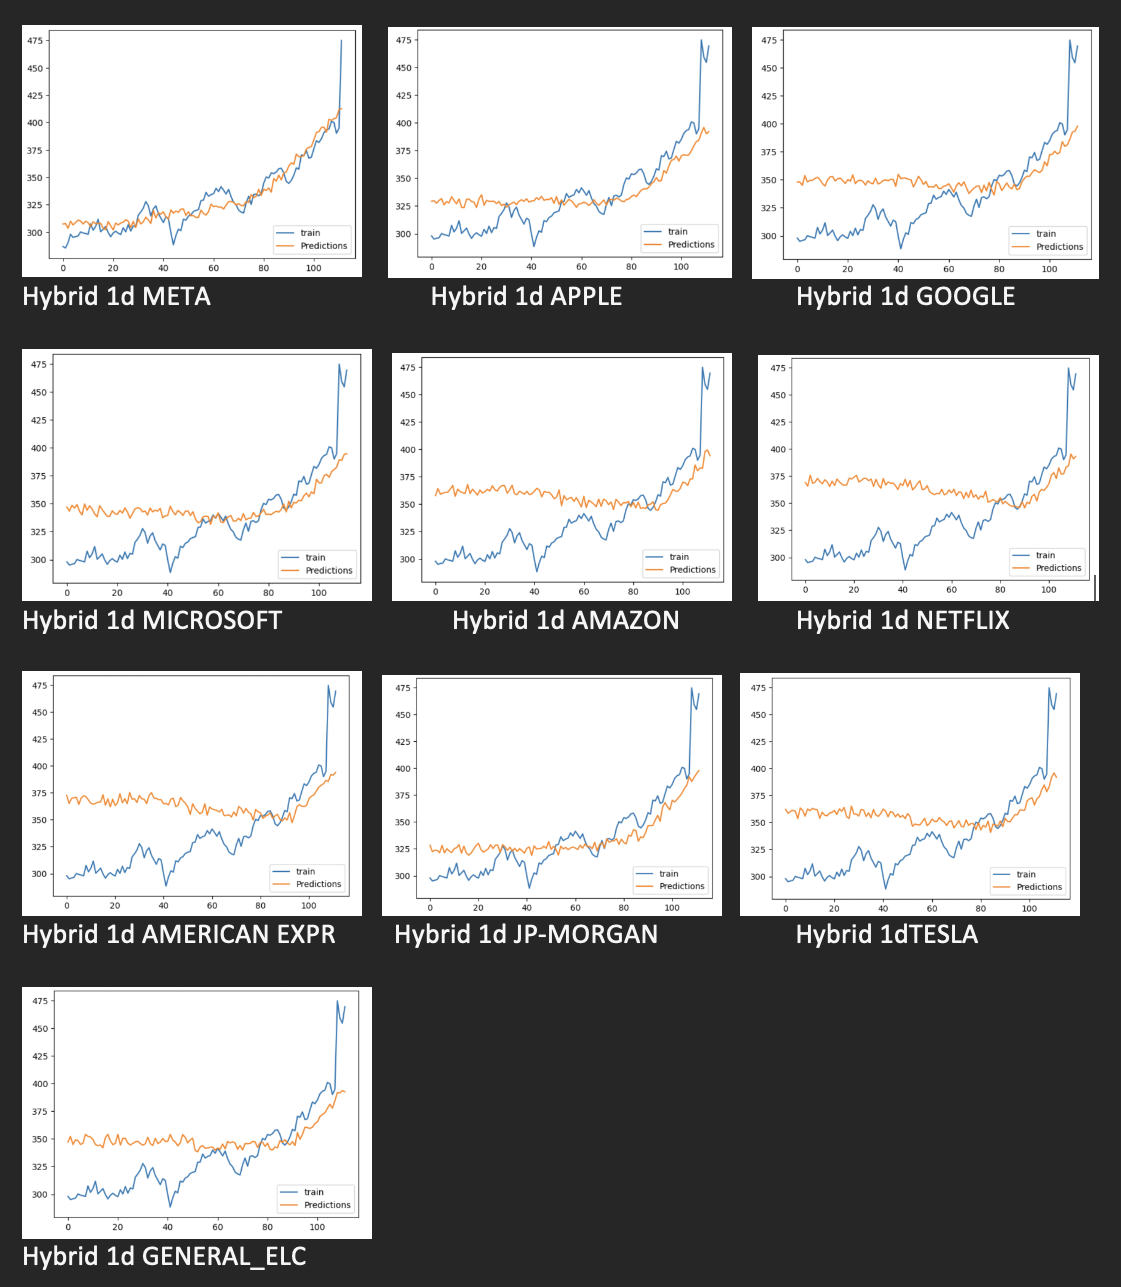
\includegraphics[scale=0.2]{figures/Hybrid 1d.png}
    \caption{Representing the overall actual and predicted values for Close stock for ARIMA-ANN algorithms with time period as 1day.}
    \label{fig:chart_e}
\end{figure}

\begin{figure}[ht]
    \centering
    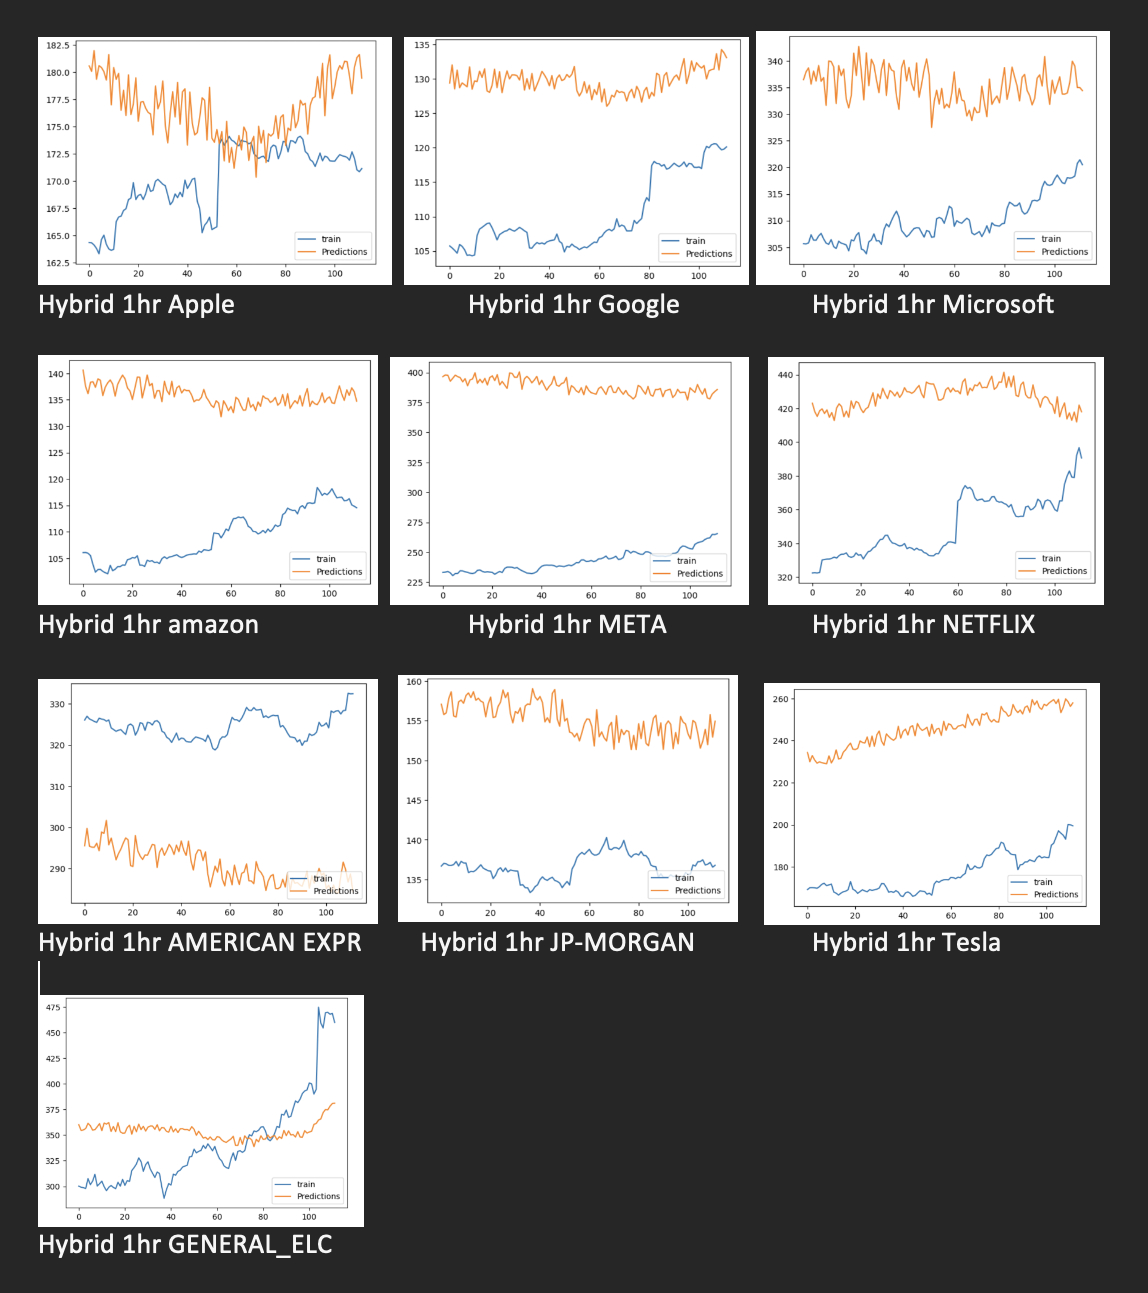
\includegraphics[scale=0.2]{figures/Hybrid 1hr.png}
    \caption{Representing the overall actual and predicted values for Close stock for ARIMA-ANN algorithms with time period as 1hr.}
    \label{fig:chart_d}
\end{figure}

The overall differences in the forecasts between the ARIMA-ANN and TNN outcomes are shown for every iteration throughout the designated time frame. The ARIMA-ANN and TNN model designs have undergone several modifications, and the interpolation methods show improvements in the overall prediction procedure, which favors TNN over ARIMA-ANN. In order to guarantee the effective loss for the design, our TNN design made use of the Dense layer, which has various functional capabilities providing overall alterations in the attentions, activation, and feedforwarding classes.

Figure 5.1 shows the total forecast values for the 10 tickers under consideration, providing a broad overview of how the predictions and actual values differ. The overall charting of these characteristics is dependent on the multi-objective function post-prediction interpolation based on the prediction with various constraints on each and every sample that is taken into consideration.



    \chapter{Discussion and Analysis}
\label{ch:evaluation}

We are able to train Yahoo finance data with the transformer neural networks and ARIMA-ANN Hybrid. We used the co-variance relations between the tickers to do the predictions. And In designing the ARIMA-ANN hybrid we first trained the ARIMA and we calculate the residual. Then we used that residual to train the ANN. Then with this trained  ANN we did the predictions of the stock price. For Transformer neural network we recored less RMSE error when compared to the ARIMA-ANN hybrid.

    \chapter{Conclusions and Future Work}
\label{ch:con}
\section{Conclusions}
Based on the average error findings in each of the selected stock prediction firms, we have effectively demonstrated in this study that our suggested TNN model is significantly better than the ARIMA-ANN hybrid. The suggested design performs better than the original plan overall and shows the optimal outcomes for a 1-hour and 5-minute time frame. To improvise such adjustments, it will be necessary to evaluate additional elements of the relative likelihood of the stock prices and yet substantial improvements on the bi-cubic interpolation technique.


\section{Future work}
When compared to the ARIMA-ANN Hybrid, the TNN architecture often offers superior average error margins. With a bi-cubic and multinominal dimensionality technique, the effective change in the time series prediction will be more effective since only dense layers were selected. In all scenarios with varying stock values, the overall design layer improvement with custom optimization layers may be applied to the design lowering the total loss less than 1%.

    \chapter{Reflection}
\label{ch:reflection}
%%%%%%%%%%%%%%%%%%%%%%%%%%%%%%%
%% Please remove/replace text below
%%%%%%%%%%%%%%%%%%%%%%%%%%%%%%%
Write a short paragraph on the substantial learning experience. This can include your decision-making approach in problem-solving.

\textbf{Some hints:} You obviously learned how to use different programming languages, write reports in \LaTeX and use other technical tools. In this section, we are more interested in what you thought about the experience. Take some time to think and reflect on your individual project as an experience, rather than just a list of technical skills and knowledge. You may describe things you have learned from the research approach and strategy, the process of identifying and solving a problem, the process research inquiry, and the understanding of the impact of the project on your learning experience and future work.

Also think in terms of:
\begin{itemize}
    \item what knowledge and skills you have developed
    \item what challenges you faced, but was not able to overcome
    \item what you could do this project differently if the same or similar problem would come
    \item rationalize the divisions from your initial planed aims and objectives.
\end{itemize}


A good reflective summary could be approximately 300--500 words long, but this is just a recommendation.

~\\[2em]
\noindent
{\huge \textbf{Note:}} The next chapter is ``\textbf{References},'' which will be automatically generated if you are using BibTeX referencing method. This template uses BibTeX referencing.  Also, note that there is difference between ``References'' and ``Bibliography.'' The list of ``References'' strictly only contain the list of articles, paper, and content you have cited (i.e., refereed) in the report. Whereas Bibliography is a list that contains the list of articles, paper, and content you have cited in the report plus the list of articles, paper, and content you have read in order to gain knowledge from. We recommend to use only the list of ``References.'' 

    

    
    % -------------------------------------------------------------------
    % Bibliography/References  -  Harvard Style was used in this report
    % -------------------------------------------------------------------
    \bibliographystyle{agsm} % Harvard Style 
    
    \bibliography{references}  %  Patashnik, O. (1988), BibTEXing. Documentation for general BibTEX users.
    
    % -------------------------------------------------------------------
    % Appendices
    % -------------------------------------------------------------------
    
    \begin{appendices}
        \chapter{An Appendix Chapter (Optional)}
\label{appn:A}
% Optional chapter
Some lengthy tables, codes, raw data, length proofs, etc. which are \textbf{very important but not essential part} of the project report goes into an Appendix. An appendix is something a reader would consult if he/she needs extra information and a more comprehensive understating of the report. Also, note that you should use one appendix for one idea.

An appendix is optional. If you feel you do not need to include an appendix in your report, avoid including it. Sometime including irrelevant and unnecessary materials in the Appendices may unreasonably increase the total number of pages in your report and distract the reader.


        \chapter{An Appendix Chapter (Optional)}
\label{appn:B}

...
    \end{appendices}
    
\end{document}
